% 阿基米德螺线
% 极坐标|阿基米德|曲线方程

\pentry{极坐标中的曲线方程\upref{PolCrd}}

\textbf{阿基米德螺线}(\autoref{ArcSpl_fig2})的极坐标方程为
\begin{equation}
r = a + b\theta \qquad (\theta > -a/b)
\end{equation}
注意虽然从原点发出的任意射线都与曲线有无穷多个交点, 但一个 $\theta$ 仍然只对应一个 $r$, 函数仍然是单值的.

\begin{figure}\label{ArcSpl_fig2}[ht]
\centering
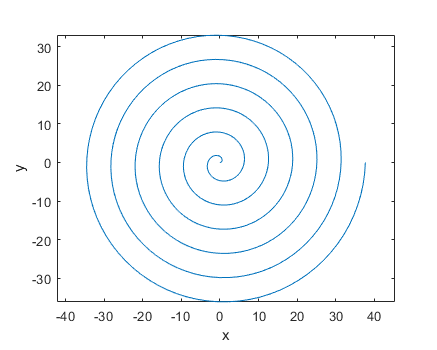
\includegraphics[width=9cm]{./figures/ArcSpl_1.png}
\caption{阿基米德螺线, $r = \theta$} \label{ArcSpl_fig1}
\end{figure}

% 图未完成
% 所以就是没有完成
% 没有完成
